\section{Transformers for Vision}

\begin{frame}{Transformers: From Language to Vision}
    \begin{itemize}
        \item The Transformer architecture was designed for \textbf{sequence-to-sequence learning}.
        \item Transformers have revolutionized NLP and become the model of choice.
        % \item In the field of \textbf{Computer Vision} however, the dominant architecture has remained the CNN.
	\item Is it possible to adapt the Transformer for image data?
    \end{itemize}
\end{frame}


\begin{frame}{Idea \#1: Add Attention to Existing CNNs}
    \begin{itemize}
        \item Model is still a CNN!
    \end{itemize}
    \begin{figure}
        \centering
        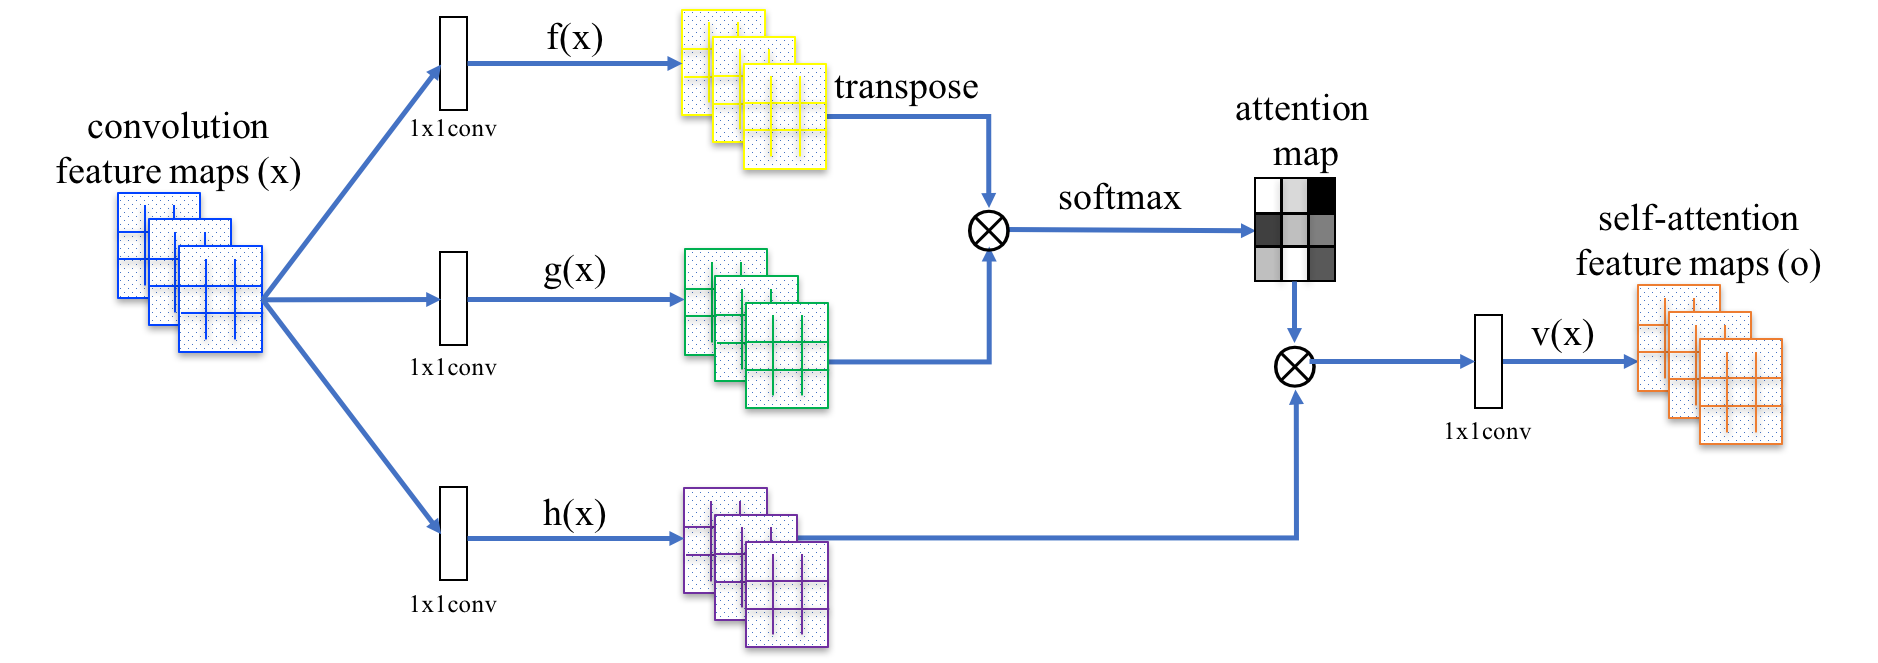
\includegraphics[width=\linewidth]{pic/framework}
        % \caption{Add Self-Attention blocks between existing ResNet blocks.}
        \label{fig:idea1}
    \end{figure}
\end{frame}

\begin{frame}{Idea \#2: Replace Convolution with “Local Attention”}
    \begin{itemize}
        \item Lots of tricky details, hard to implement, only marginally better than ResNets.
    \end{itemize}
    \begin{figure}
        \centering
        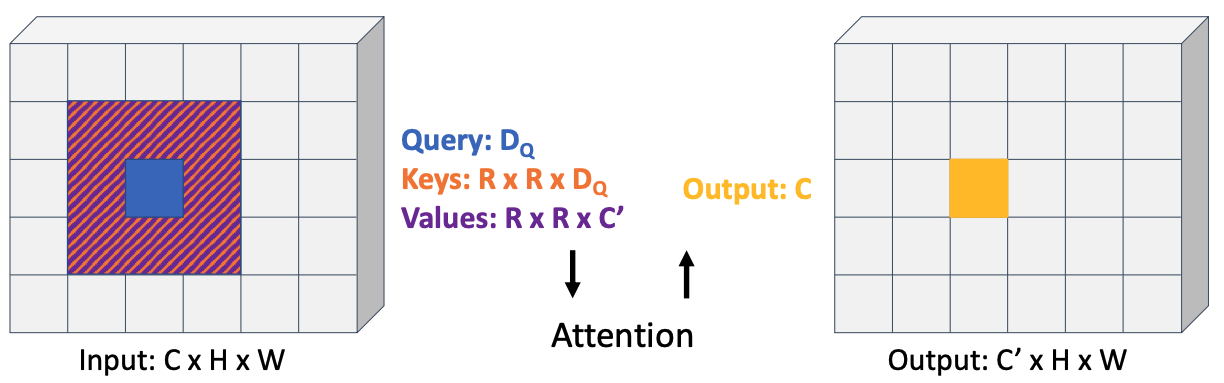
\includegraphics[width=\linewidth]{pic/idea2}
        % \caption{Replace all convolutional layers in CNNs with local attention.}
        \label{fig:idea1}
    \end{figure}
\end{frame}


\begin{frame}{Idea \#3: Standard Transformers on Pixels}
    \begin{itemize}
        \item Insane memory usage!
    \end{itemize}
    \begin{figure}
        \centering
        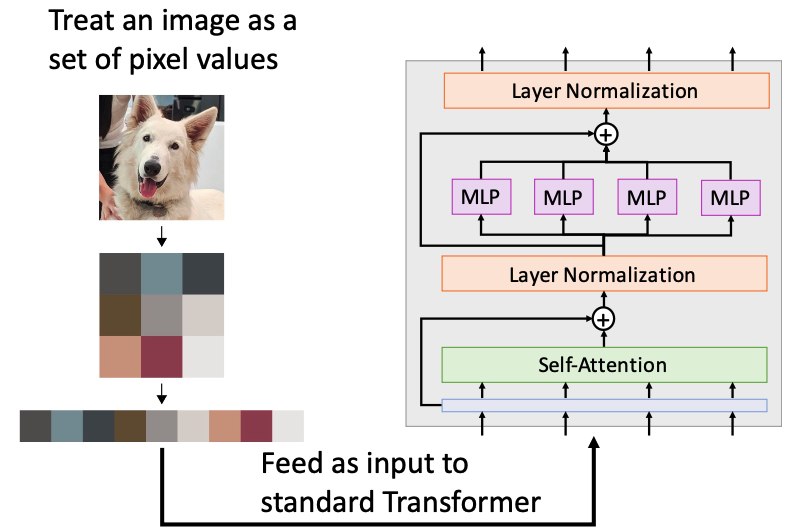
\includegraphics[width=0.5\linewidth]{pic/idea3}
        % \caption{Treat each image pixel as an input token for the transformer.}
        \label{fig:idea1}
    \end{figure}
\end{frame}


\begin{frame}{Idea \#4: Standard Transformer on Patches}
    \begin{itemize}
        % \item Follow the original Transformer as closely as possible.
        \item Fixes idea \#1 by entirely replacing convolutional layers.
        \item Fixes idea \#2 by simplifying implementation.
        \item Fixes idea \#3 by reducing memory usage.
        \item This is the main idea behind \textbf{Vision Transformers}!
    \end{itemize}
\end{frame}
